\setcounter{listing}{0}

\section{Implementacja systemu}

W tym rozdziale opisana została implementacja systemu. Na początku omówiono sposób działania aplikacji internetowej oraz mobilnej na przykładowych fragmentach kodu. Dalsza część zawiera wyniki działania systemu, w tym zrzuty ekranu aplikacji mobilnej. Na końcu znajdują się metody testowania systemu oraz środowiska programistyczne i edytory wykorzystane do realizacji zadań pracy.

\subsection{Aplikacja internetowa}

Główne zadania jakie były do zrealizowania podczas implementacji serwera, to: autoryzacja, zarządzanie i identyfikowanie pojazdów, kupno oraz kontrola biletu postojowego. Aby te funkcjonalności mogły być osiągalne dla aplikacji mobilnej, konieczne jest udostępnienie zasobów poprzez adresy URL. W Django razem z projektem tworzony jest plik urls.py, gdzie są one umieszczane w liście urlpatterns. Każda pozycja to wywołanie funkcji ulr(), która jako pierwszy argument przyjmuje wyrażenie regularne z adresem, a jako drugi widok, który obsługuje żądanie.
\\
\\
Na listingu \ref{parq_urls} zaprezentowany jest fragment kodu z pliku urls.py, ze wszystkimi adresami na jakie swoje żądania wysyła aplikacja mobilna. W zależności od realizowanych zadań, przyjmują wybrane metody protokołu HTTP.

\begin{singlespace}
	\captionof{listing}{Mapowane adresy URL z pliku urls.py}
	\label{parq_urls}
	\vspace{0.3cm}
	\inputminted[fontsize=\footnotesize, linenos=true]{python}{src/imp/urlpatterns.py}
\end{singlespace}

\subsubsection*{Tworzenie konta i autoryzacja}

Z procesem utworzenia konta w systemie przez kierowcę lub kontrolera związanych jest kilka dodatkowych czynności. Są to przypisanie roli oraz generowanie tokenu autoryzacyjnego. Wszyscy użytkownicy tworzeni są w oparciu o istniejący już w Django model użytkownika -- User, z modułu django.contrib.auth.models. Niezbędny jest jednak sposób, który pozwoli na odróżnienie kierowcy od kontrolera, aby można było nadać im odmienne uprawnienia. Do tego celu wykorzystany został dodatek djroles, napisany specjalnie na potrzeby tego systemu. Swoje działanie opiera na istniejących w Django grupach, z którymi domyślnie użytkownicy są w relacji wiele-do-wielu. Dodatek ten tworzy dodatkową tabelę -- Role, w której umieszczane są wybrane grupy. Spośród nich, użytkownik będzie mógł należeć tylko do jednej, w tym samym czasie. Na listingu \ref{driver} pokazany został sposób, w jaki są deklarowane grupy, które będą używane do tworzenia ról. Jest to robione poprzez zadeklarowanie klasy Pythona, która dziedziczy po BaseRole - jej nazwa zostanie użyta do utworzenia grupy. Jako że ten język dopuszcza wielodziedziczenie, wykorzystany został model Driver oraz Officer, dzięki czemu grupa posiada tę samą nazwy co tabele z dodatkowymi informacjami kierowcy i kontrolera.

\begin{singlespace}
	\captionof{listing}{Fragment modelu Driver}
	\label{driver}
	\vspace{0.3cm}
	\inputminted[fontsize=\footnotesize, linenos=true]{python}{src/imp/driver.py}
\end{singlespace}

\vspace{0.3cm}

Poza przypisaniem grupy, każdy użytkownik w systemie, niezależnie już od pełnionej roli, musi mieć wygenerowany token autoryzacyjny. Obie te czynności realizowane są przez sygnały (ang. signals), dostępne w Django. Są to funkcje, które zostaną wykonane w odpowiedzi na jakieś zdarzenie związane z ustaloną klasą w projekcie. Na listingu \ref{sygnaly} przedstawione zostały sygnały powiązane z domyślną klasą użytkownika User (tworzenie tokenu) oraz klasami Driver i Officer -- przypisywanie do ról. Wykonywane są w odpowiedzi na zapisanie modelu w bazie danych, czyli sygnał post\_save.

\begin{singlespace}
	\captionof{listing}{Sygnały związane z tworzeniem konta w systemie}
	\label{sygnaly}
	\vspace{0.3cm}
	\inputminted[fontsize=\footnotesize, linenos=true]{python}{src/imp/token_signal.py}
\end{singlespace}

\subsubsection*{Identyfikacja pojazdów}

Z każdym pojazdem kierowcy w systemie powiązany jest identyfikator UUID (ang. Universally unique identifier), czyli 128-bitowa losowa wartość. Przechowywana jest ona w modelu Badge (listing \ref{model_badge}), powiązanym relacją jeden-do-jeden z pojazdem (Vehicle). W modelu znajduje się także metoda generate\_image(). W niej właśnie utworzony zostanie kod QR, w którym zakodowany będzie identyfikator. Do generowania QR w postaci pliku png, użyta została biblioteka Pythona qrcode. Oprócz danych, podawany jest także poziom korekcji błędów i wersja kodu.

\begin{singlespace}
	\captionof{listing}{Badge - model identyfikatora}
	\label{model_badge}
	\vspace{0.3cm}
	\inputminted[fontsize=\footnotesize, linenos=true]{python}{src/imp/badges-badge.py}
\end{singlespace}

\vspace{0.3cm}

Utworzony w ten sposób kod QR jest następnie wysyłany na e-maila, podanego przez kierowcę podczas rejestracji. Umieszczony w widocznym miejscu pojazdu, będzie używany przez kontrolera podczas sprawdzania biletu.

\subsubsection*{Taryfikator}

Taryfikator oprócz powiązanych ze sobą opłat, musi zawierać także informację o czasie w którym obowiązuje, zarówno godzin jak i konkretnej daty w kalendarzu. Dobrym rozwiązaniem jest umożliwienie ustawienia także takiej daty jako cyklicznej, dzięki czemu dany taryfikator mógłby obowiązywać np.: co tydzień w sobotę. Taką możliwość daje klasa Event, z dodatku django-scheduler. Pozwala ona na stworzenie wydarzenia z datą początkową oraz końcową, która będzie przechowywana w bazie danych. Dodatkowo takie wydarzenie może być cykliczne, a podane daty wyznaczać będą wtedy dzień tygodnia, czy miesiąca. Model Schedule rozszerza Event, dzięki czemu taryfikator posiada zarówno opłaty jak i czas obowiązywania. Na listingu \ref{schedule-create} przedstawiono przykład jego tworzenia.

\begin{singlespace}
	\captionof{listing}{Tworzenie cotygodniowego taryfikatora}
	\label{schedule-create}
	\vspace{0.3cm}
	\inputminted[fontsize=\footnotesize, linenos=true]{python}{src/imp/schedule-create.py}
\end{singlespace}


\subsubsection*{Kupno biletu}

Oprócz pojazdu na jaki ma zostać zakupiony bilet, użytkownik podaje także parking, który razem z datą rozpoczęcia postoju wyznacza obowiązujący taryfikator. Podobnie jak w Strefie Płatnego Parkowania w Szczecinie, cena może się zmieniać w zależności od długości parkowania. Na listingach \ref{calculate-schedule} i \ref{calculate-charge} przedstawione zostały algorytmy naliczające opłatę. W klasie Schedule najpierw wyznaczany jest efektywny czas postoju, w przypadku gdyby podany bilet wykraczał poza datę obowiązywania taryfikatora. Po przedstawieniu czasu trwania postoju w postaci minut, pobierane są wszystkie opłaty powiązane z danym taryfikatorem. Następnie w pętli, aż do wyczerpania ilości minut postoju, każda z opłat nalicza swoją część ceny (model Charge), zgodnie z jej czasem obowiązywania. W przypadku wyczerpania listy opłat przed zakończeniem postoju, ostatnia z nich (tak jak w SPP w Szczecinie) naliczy cenę dla pozostałych minut postoju. W pętli wszystkie opłaty cząstkowe są sumowane i ta właśnie suma zostanie naliczona jako opłata kierowcy.

\begin{singlespace}
	\captionof{listing}{Obliczanie łącznej kwoty w klasie Schedule}
	\label{calculate-schedule}
	\vspace{0.3cm}
	\inputminted[fontsize=\footnotesize, linenos=true]{python}{src/imp/schedule-calculate_price.py}
\end{singlespace}

\begin{singlespace}
	\captionof{listing}{Obliczanie częstki ceny w pojedynczej opłacie - model Charge}
	\label{calculate-charge}
	\vspace{0.3cm}
	\inputminted[fontsize=\footnotesize, linenos=true]{python}{src/imp/charge-calculate_price.py}
\end{singlespace}

\subsubsection*{Doładowanie konta}

%TODO sprawdzaj czy podane linie się zgadzają!
Doładowywanie konta odbywa się dwustopniowo. Najpierw w aplikacji mobilnej użytkownik przelewa swoje pieniądze (np.:~z wykorzystaniem karty płatniczej) na konto PayPal'a powiązane z systemem. Zwrócony identyfikator transakcji wysyłany jest metodą POST do serwera systemu ParQ, na adres payments/. W widoku przedstawionym na listingu \ref{payments_list}, obsługującym ten adres, przedstawiony jest fragment kodu odpowiedzialny za to żądanie. W linii 12 wywoływana jest metoda, w której otrzymany identyfikator przesyłany zostaje do serwera PayPal'a, celem uzyskania informacji o kwocie jaka została przelana. Następnie, jeśli wszystko się zgadza, numer transakcji zapisywany jest w bazie danych (linia 13). Gdy transakcja o takim identyfikatorze już istnieje, zwrócony zostanie w odpowiedzi błąd. Tylko w razie powodzenia wykonana będzie następna linia, gdzie powiązana portmonetka użytkownika jest uzupełniana o wpłaconą kwotę.

\begin{singlespace}
	\captionof{listing}{payment\_list - widok doładowania konta użytkownika}
	\label{payments_list}
	\vspace{0.3cm}
	\inputminted[fontsize=\footnotesize, linenos=true]{python}{src/imp/paypal-views.py}
\end{singlespace}

\vspace{0.3cm}

Do realizacji tej części pracy wykorzystano kilka dodatków do Django oraz jeden dodatkowy pakiet Pythona, a są to:
\begin{itemize}
	\item Django REST Framework -- na jego podstawie tworzone są widoki, które obsługują żądania w architekturze REST. Ten dodatek umożliwia także autoryzacje żądań, opartą na generowanym wcześniej tokenie.
	\item django-scheduler -- tworzenie wydarzeń, które mogą się powtarzać cyklicznie.
	\item django-ordered-model -- numerowane relacje w tabelach.
	\item django-countries -- państwa i ich kody ze standardu ISO 3166.
	\item djroles -- tworzenie ról w Django.
	\item qrcode -- pakiet Pythona umożliwiający generowanie kodów QR.
\end{itemize}

\subsection{Aplikacje mobilne}

W ramach pracy zostały wykonane dwie oddzielne aplikacje dla kierowcy oraz kontrolera, ze względu na odmienny sposób w jaki korzystają oni z systemu. Kierowca oprócz logowania, powinien móc m.in. założyć konto, czy dokonać płatności przy doładowywaniu konta. Kontroler w swojej aplikacji powinien mieć możliwość przeprowadzenia kontroli biletów postojowych, co odbywa się poprzez odczytanie plakietki z kodem QR. Do każdej z tych aplikacji zalogować może się jedynie użytkownik posiadający konto, do którego została przypisana odpowiednia rola. Obie wymagają ciągłej komunikacji z serwerem.

\subsubsection*{Parsowanie danych}

Format JSON składa się z par danych - z każdą wartością związany jest klucz, który służy do jej identyfikacji. Przechowywana wartość może być ciągiem znaków, liczą całkowitą i zmiennopozycyjną, ale także obiektem zawierającym dalszy zestaw par (otoczonym nawiasami klamrowymi) lub tablicą takich obiektów (nawiasy klamrowe). JSON przesyłany jest jako tekst w części danych żądania lub odpowiedzi HTTP. W celu wydobycia informacji musi być poddany odpowiedniej analizie, zarówno na serwerze jak i aplikacji mobilnej. W Androidzie parsowanie można wykonać za pomocą klas JSONObject oraz JSONArray z pakietu org.json 
\\
\\
JSONObject umożliwia parsowanie pojedynczego jsona, a dane do analizy podawane są jako ciąg znaków (String) w konstruktorze. Metody instancji tej klasy służące do wydobywania wartości, jako parametr przyjmują nazwę klucza z jakim ta wartość jest związana. Są to m.in: get(), getInt(), czy getString(), a ich użycie zależy od spodziewanego typu wartości przechowywanego w dokumencie. Istnieje także metoda getJSONObject(), która zwraca zagnieżdżony obiekt jsona w postaci instancji klasy JSONObject. JSONArray instancjonowana jest w podobny sposób, a używana jest w przypadku gdy json zawiera tablicę danych. Po wywołaniu metody getJSONObject() z indeksem elementu w parametrze, zwracany jest obiekt pojedynczego jsona, czyli klasy JSONObject. Na listingu \ref{parsowanie} znajduje się przykład z wykorzystaniem kolekcji danych.

\begin{singlespace}
	\captionof{listing}{Parsowanie jsona dla kolekcji pojazdów kierowcy}
	\label{parsowanie}
	\vspace{0.3cm}
	\inputminted[fontsize=\footnotesize, linenos=true]{java}{src/imp/parsowanie-json.java}
\end{singlespace}

Ten fragment kodu zostaje wykonany, w momencie otrzymania z serwera pojazdów powiązanych z danym kierowcą. Dla każdego elementu tablicy json wydobywany jest obiekt klasy JSONObject, z którego pobierane są dane pojazdu. Zostaną one później zaprezentowane użytkownikowi w odpowiednim widoku.

\subsubsection*{Komunikacja z serwerem}

Komunikacja w systemie polega na wysyłaniu żądań przez aplikacje do serwera i oczekiwaniu na rezultat, który zostanie przesłany w odpowiedzi. Tym zajmuje się biblioteka HTTP -- Volley. Stanowi alternatywę dla wykorzystywanych wcześniej klas Javy, jak HttpURLConnection, będąc rozwiązaniem dedykowanym dla Androida, cechującym się prostotą i szybkością działania. Świetnie nadaje się do prostych API, w których wymiana informacji polega na przesyłaniu list oraz pojedynczych danych w formacie json. Jedną z jej głównych zalet jest zdolność do buforowania odpowiedzi. Jeśli zapytanie może zostać obsłużone dzięki danych znajdującym się w pamięci podręcznej, nie będzie ono musiało zostać ponownie wysłane.
\\
\\
Listing \ref{volley} przedstawia sposób, w jaki konstruowane są zapytania w tej bibliotece. Najpierw w konstruktorze podawany jest rodzaj metody HTTP oraz adres, na jaki żądanie będzie miało zostać wysłane. Dwa następne parametry to obiekty klas anonimowych. Jeśli odpowiedz z serwera będzie zwrócona z kodem 2xx, to wykonana zostanie metoda onResponse() pierwszego obiektu. Parametr response zawiera dane odpowiedzi i to właśnie on będzie poddawaniu parsowaniu. Jeśli odpowiedz jest błędna, czyli wysłana została z kodem 4xx lub 5xx, wykonana zostanie onErrorResponse. Tak utworzone zapytanie dodawane jest do kolejki zapytań, gdzie kolejność wysłania może być zależna od ustawionego priorytetu.

\begin{singlespace}
	\captionof{listing}{Wysłanie żądania}
	\label{volley}
	\vspace{0.3cm}
	\inputminted[fontsize=\footnotesize, linenos=true]{java}{src/imp/scan-activity.java}
\end{singlespace}

\subsubsection*{Realizacja płatności}

Do integracji PayPal'a z aplikacją mobilną została wykorzystana biblioteka PayPal Android SDK, która jest dostępna w ramach open source. Razem z nią, oprócz możliwości realizacji opłat, udostępniane są także gotowe ekrany, gdzie użytkownik może podać swoje dane uwierzytelniające. Biblioteka ta pozwala na realizowanie płatności pojedynczych (tzw. Single Payment, użytkownik za każdym razem musi podawać dane uwierzytelniające) oraz automatycznych (Future Payment, dane podawane tylko raz, a zwrócony token OAuth pozwala na dokonywanie płatności w imieniu użytkownika). W tym systemie oferowana jest tylko pierwsza opcja.
\\
\\
Na listingu \ref{paypal1} przedstawiony został fragment, w którym za pomocą intencji uruchomiona zostaje aktywność uwierzytelnienia płatności. W klasie PayPalPayment podawane zostają informacje odnośnie wysokości płatności, waluty oraz typu transakcji. Obiekt tej klasy, razem z informacjami konfiguracyjnymi, zostaje umieszczony w intencji. Wywołanie metody aktywności Androida startActivityForResult() spowoduje wyświetlenie nowego ekranu.

\begin{singlespace}
	\captionof{listing}{Intencja rozpoczynająca aktywność PayPal'a}
	\label{paypal1}
	\vspace{0.3cm}
	\inputminted[fontsize=\footnotesize, linenos=true]{java}{src/imp/get-payment.java}
\end{singlespace}

Metoda startAcitvityForResult() uruchamiająca nową aktywność różni się od startActivity() tym, że od docelowej aktywności oczekiwane jest otrzymanie jakiegoś wyniku. Po zakończeniu utworzonego ekranu uruchomiona zastanie metoda onActivityResult(). Do niej właśnie przesłana zostanie odpowiedź z serwera PayPal'a o statusie przeprowadzonej płatności, a także w razie sukcesu, identyfikator płatności. W tym miejscu właśnie będzie on wysłany do serwera systemu, celem jego dalszego uwierzytelnienia.

\subsubsection*{Kontrola biletu}

Kontrola biletu możliwa jest w aplikacji przeznaczonej dla kontrolera. Odbywa się poprzez skanowanie obrazu z kamery wbudowanej w urządzenie mobilne. Do tego celu użyta została biblioteka ZXing ("Zebra Crossing"), która służy do przetwarzania obrazu. Oprócz QR, umożliwia także skanowanie kodów kreskowych. Domyślnie nie są dołączone do niej żadne gotowe aktywności, jak w przypadku PayPal Android SDK. Istnieje jednak dodatek, ZXing Android Embedded, którego sposób działania jest zbliżony do przeprowadzania transakcji. Zawiera on gotową aktywność, w której zostaje uruchomiona kamera urządzenia mobilnego. Na listingu \ref{platnosc} w klasie IntentIntegrator konfigurowany jest najpierw skaner. Podawany jest tam rodzaj kodów graficznych, czy orientacja ekranu. Po natrafieniu przez skaner na kod, skanowanie zostaje zakończone. Informacja jaką udało się odkodować, zwracana jest w metodzie onActivityResult().

\begin{singlespace}
	\captionof{listing}{Intencja rozpoczynająca aktywność skanowania}
	\label{platnosc}
	\vspace{0.3cm}
	\inputminted[fontsize=\footnotesize, linenos=true]{java}{src/imp/start-scan.java}
\end{singlespace}

Po zeskanowaniu kodu, znajdująca się w nim informacja trafia do serwera. Tam sprawdzane jest najpierw, czy jest to poprawny identyfikator UUID. Wykorzystane do tego zostało odpowiednie wyrażenie regularne. Następnie, jeśli format jest poprawny, wykonywane są zapytania do bazy danych, mające na celu znalezienie tego kodu, powiązanego z nim pojazdu oraz biletu, który jest ważny. Jeśli wszystkie te operacje zakończą się sukcesem, kontroler otrzymuje informację o ważnym bilecie postojowym. W przypadku gdyby któryś z kroków zakończył się niepowodzeniem, konieczne będzie wystawienie mandatu. 

\newpage

\subsection{Wyniki działania systemu}

Kierowca korzystający z systemu ParQ, oprócz logowania i rejestracji, może także doładować konto, dodawać nowe pojazdy oraz kupować bilety postojowe w przeznaczonej dla niego aplikacji. Kontroler natomiast ma możliwość przeprowadzenia kontroli zaparkowanego pojazdu z wykorzystaniem wbudowanego w telefon aparatu. Poniżej znajduje się opis funkcjonującego systemu, z zrzutami ekranów stworzonych na jego potrzeby aplikacji mobilnych oraz wynikami działania serwera.
\\
\\
W pierwszej kolejności opisana została aplikacja przeznaczona dla kierowcy, korzystającego ze strefy płatnego parkowania. Po zalogowaniu do niej, wyświetlany jest ekran główny, znajdujący się na rys. 5.1. To tutaj użytkownik uzyskuje podstawowe dane powiązane ze swoim kontem, takie jak ilość pieniędzy znajdujących się w portmonetce, czy godziny płatnego postoju w dniu sprawdzania. Tutaj też są wyświetlane informacje o wszystkich aktywnych biletach postojowych, wraz z informacjami o pojeździe na który zostały zakupione i godziną zakończenia. Z ekranu głównego możliwe jest przejście do pozostałych ekranów aplikacji. Po naciśnięciu ikonki w lewym górnym rogu, wysuwa się menu boczne przedstawione na rys. 5.2. Na górze wyświetlana jest nazwa oraz e-mail zalogowanego użytkownika. Poniżej znajdują się opcje przenoszące do ekranów zakupu biletu, zarządzania pojazdami lub doładowywania konta.

\begin{figure}[h]
	\centering
	\begin{minipage}[b]{0.25\textwidth}
		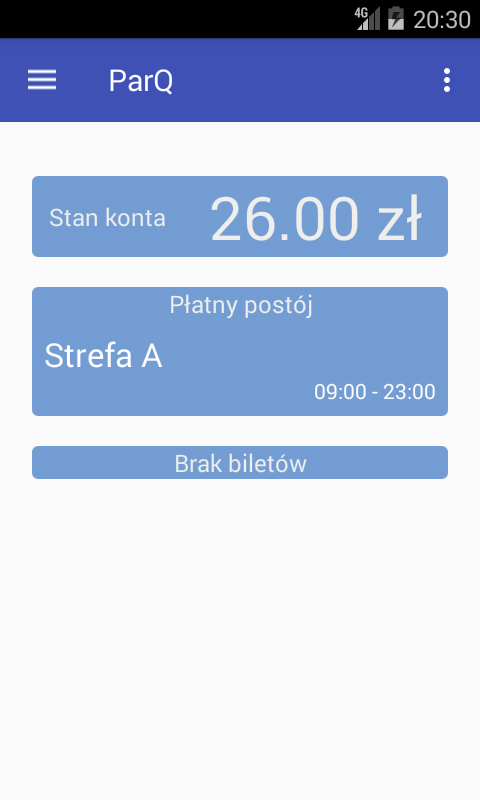
\includegraphics[width=\textwidth]{05/driver_dashboard3}
		\caption{Informacje o koncie}
	\end{minipage}
	%\hfill
	\hspace{3cm}
	\begin{minipage}[b]{0.25\textwidth}
		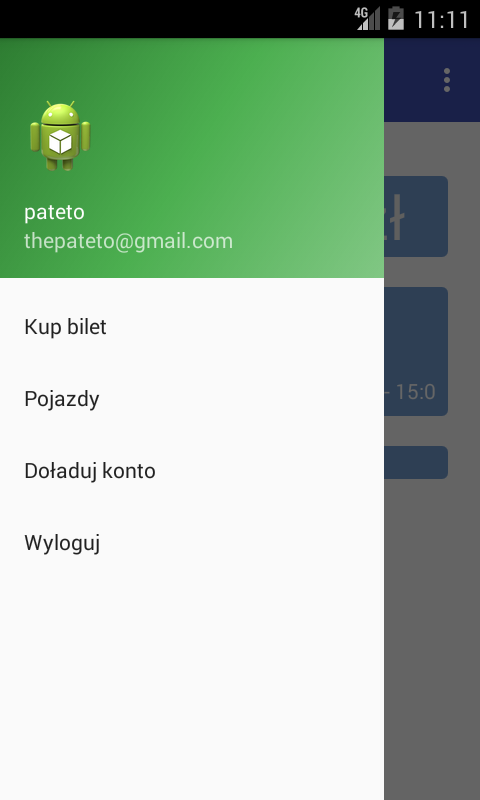
\includegraphics[width=\textwidth]{05/driver_drawer}
		\caption{Menu boczne aplikacji}
	\end{minipage}
\end{figure}

Doładowywanie konta (rys. 5.3 i 5.4) rozpoczyna się od podania kwoty, jaką konto użytkownika w systemie ma zostać doładowane. Zatwierdzenie jej, powoduje pokazanie ekranów pochodzących z wykorzystywanej do realizacji płatności biblioteki -- PayPal Android SDK. To w nich możliwe jest wybranie metody płatności, uwierzytelnienie oraz zatwierdzenie transakcji. Po zakończeniu, użytkownik przenoszony jest na ekran główny z zaktualizowanym stanem konta.

\newpage

\begin{figure}[h!]
	\centering
	\begin{minipage}[b]{0.25\textwidth}
		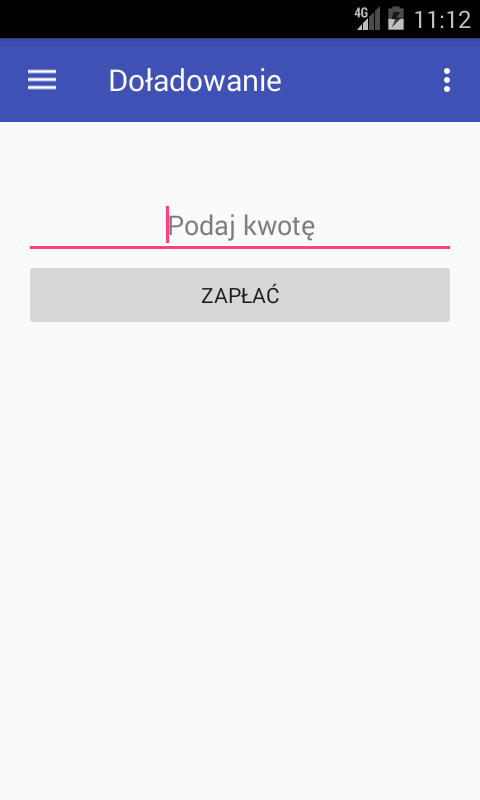
\includegraphics[width=\textwidth]{05/driver_doladowanie}
		\caption{Pole z kwotą doładowania}
	\end{minipage}
	%\hfill
	\hspace{3cm}
	\begin{minipage}[b]{0.25\textwidth}
		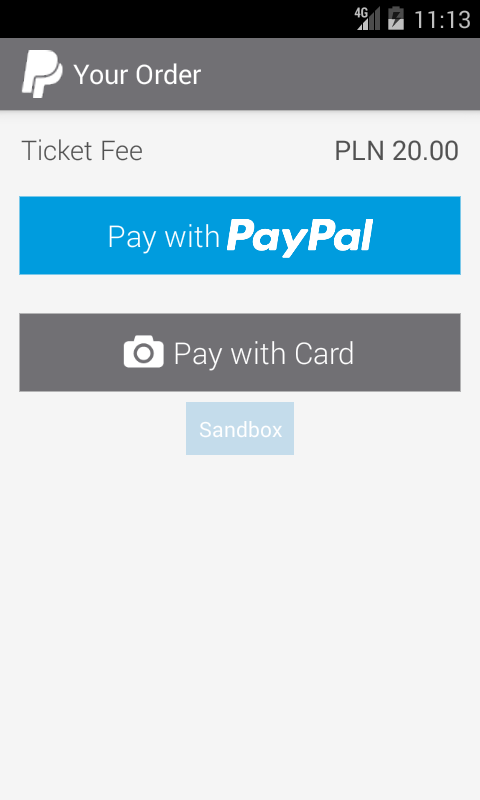
\includegraphics[width=\textwidth]{05/driver_paypal1}
		\caption{Realizacja płatności w PayPal}
	\end{minipage}
\end{figure}

Do zakupu biletu w systemie niezbędna jest informacja o pojeździe oraz parkingu, w którym będzie odbywał się postój. Te czynności wykonywane są na dwóch ekranach zaprezentowanych poniżej. Wybranie samochodu na rys. 5.5 spowoduje wyświetlenie ekranu z rys. 5.6, gdzie należy wskazać parking oraz czas postoju w minutach. Gdy użytkownik posiada odpowiednią ilość pieniędzy, nastąpi zakupienie biletu, czego potwierdzenie znajdzie się na ekranie głównym aplikacji.

\begin{figure}[h!]
	\centering
	\begin{minipage}[b]{0.25\textwidth}
		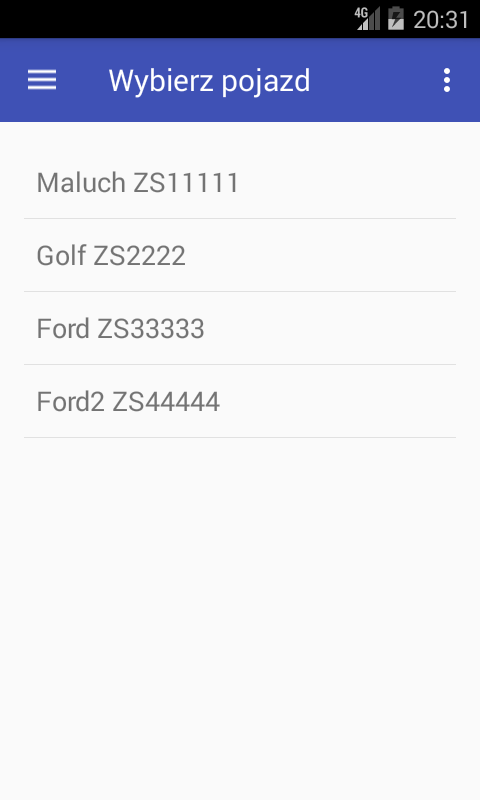
\includegraphics[width=\textwidth]{05/driver_kup_bilet1}
		\caption{Zakup biletu - wybór pojazdu}
	\end{minipage}
	%\hfill
	\hspace{3cm}
	\begin{minipage}[b]{0.25\textwidth}
		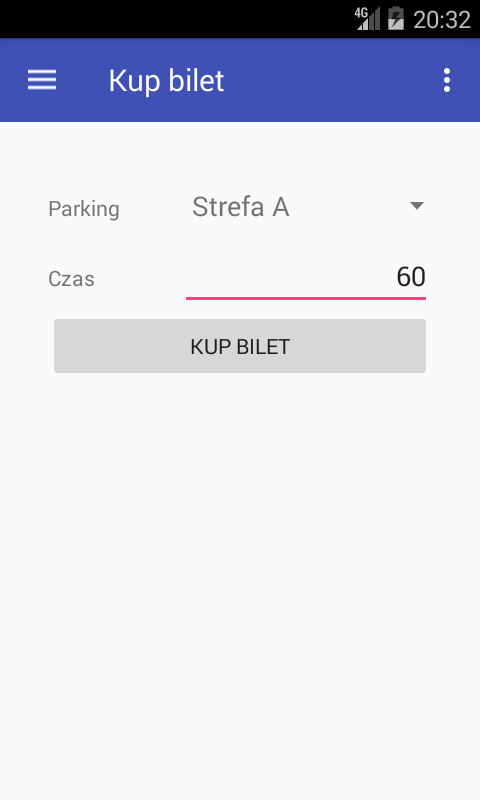
\includegraphics[width=\textwidth]{05/driver_kup_bilet2}
		\caption{Zakup biletu - parking i czas}
	\end{minipage}
\end{figure}

Na rys. \ref{przejscia_kierowca} znajduje się schemat, na którym przedstawione zostały wszystkie ekrany oraz możliwe przejścia między nimi w aplikacji przeznaczonej dla kierowców.

\newpage

\begin{figure}[h!]
	\begin{center}
		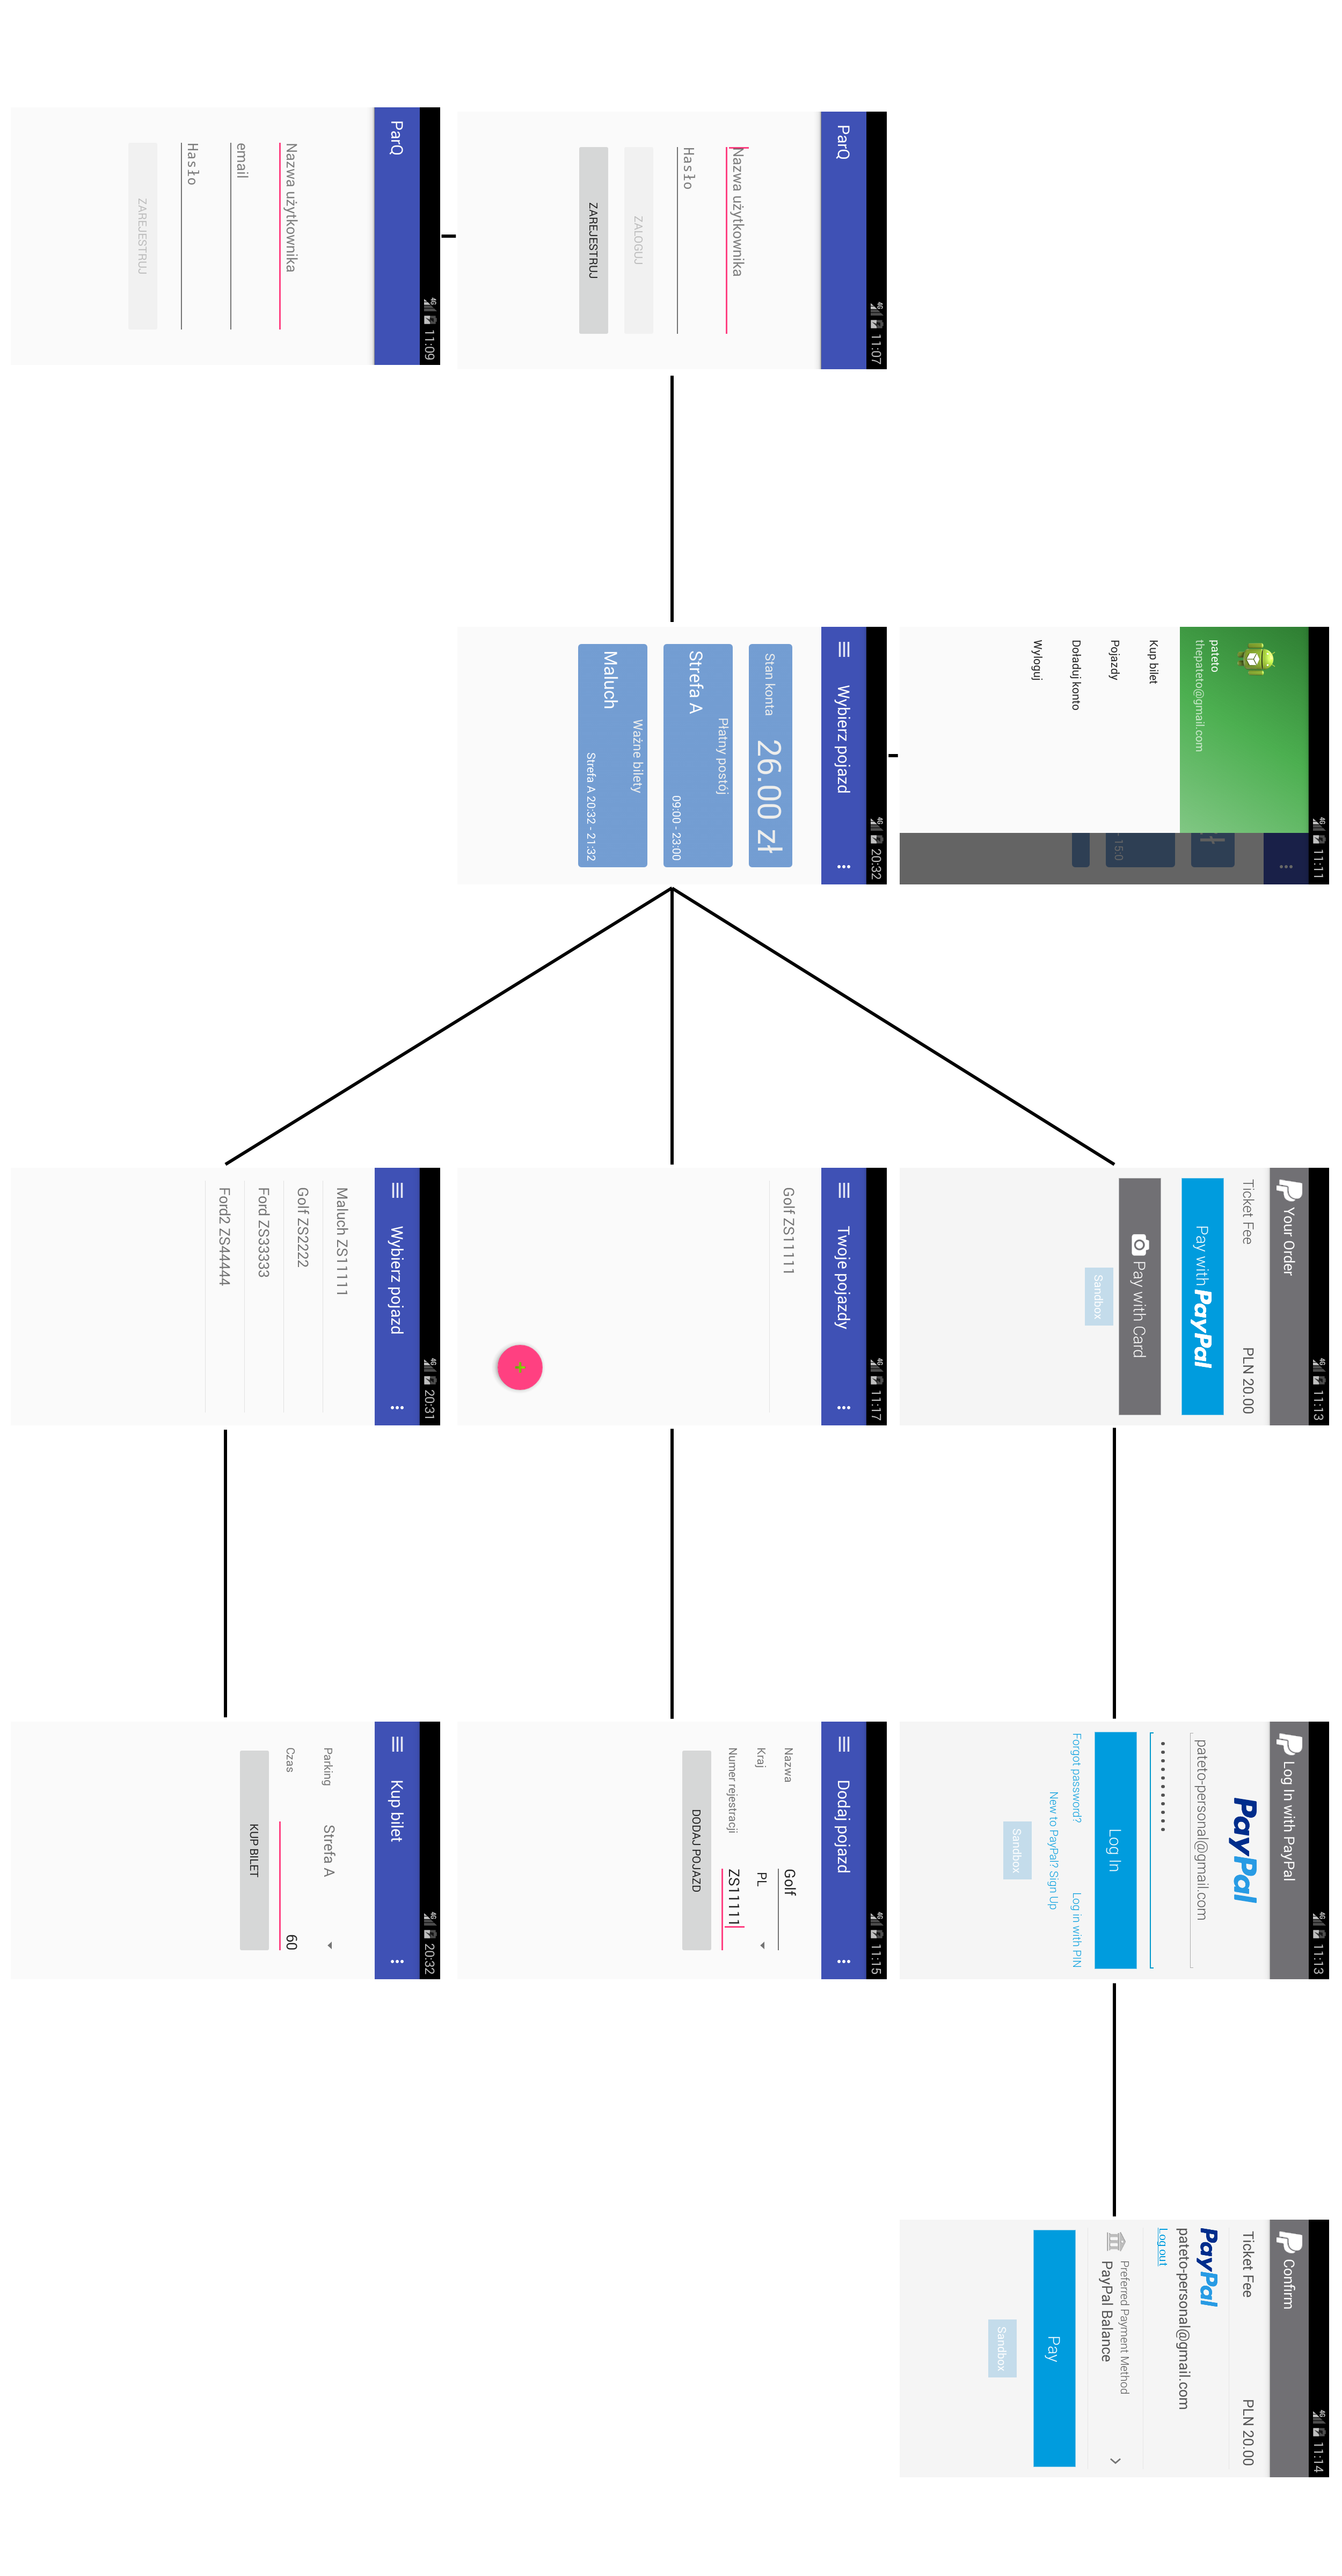
\includegraphics[width=0.7\linewidth]{05/all}
	\end{center}
	\caption{Ekrany w aplikacji kierowcy}
	\label{przejscia_kierowca}
\end{figure}

\newpage

Druga z aplikacji umożliwiająca przeprowadzenie kontroli, została zbudowana z trzech ekranów. Po zalogowaniu, użytkownikowi prezentowany jest widok, na którym będą wyświetlane informacje o kontrolowanym pojeździe. Włączenie aparatu telefonu i rozpoczęcie przeprowadzania kontroli, zaczyna się w momencie dotknięcia przycisku ``Skanuj''. W chwili napotkania dowolnego kodu QR, skanowanie zostaje zakończone, a dane znajdujące się w kodzie są wysyłane do serwera systemu. Zwrócona odpowiedź jest prezentowana na ekranie, który był widoczny zaraz po zalogowaniu. To tutaj kontroler zostanie poinformowany o tym, czy kod jest poprawny i czy jest z nim powiązany obowiązujący bilet. W celu dalszej weryfikacji, prezentowana jest także informacja o numerze rejestracyjnym, aby można było sprawdzić czy plakietka z kodem QR jest powiązana z zaparkowanym pojazdem. Na rys. \ref{przejscia_kontroler} znajdują się ekrany aplikacji kontrolera.

\begin{figure}[h!]
	\begin{center}
		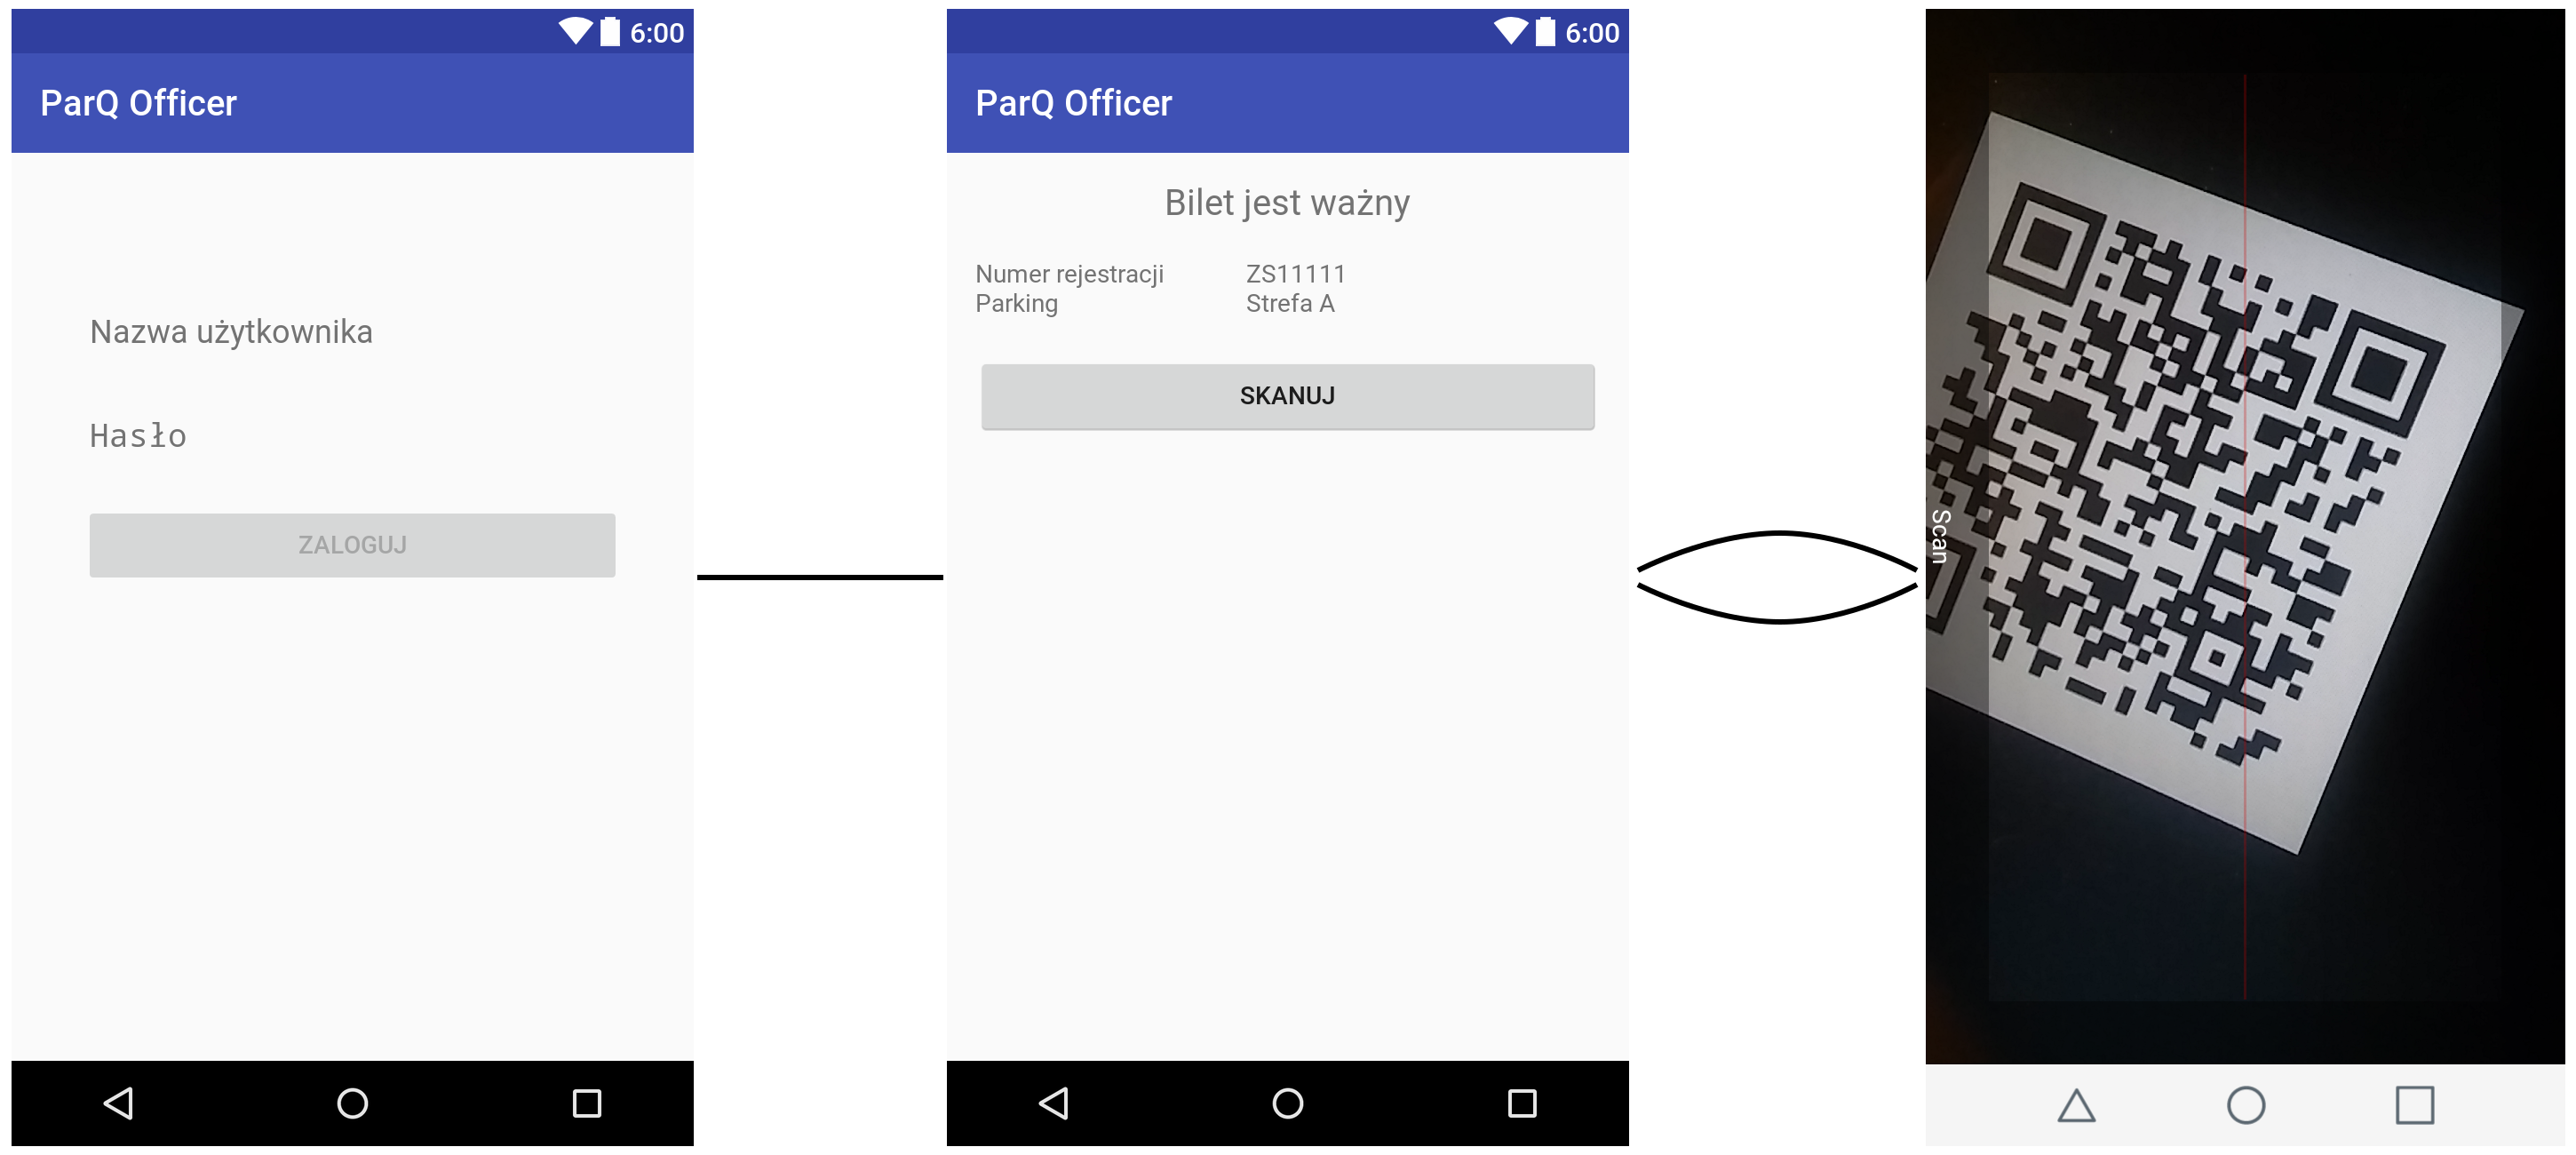
\includegraphics[width=0.7\linewidth]{05/all_officer}
	\end{center}
	\caption{Ekrany w aplikacji kontrolera}
	\label{przejscia_kontroler}
\end{figure}

Cała funkcjonalność systemu dostępna z poziomu aplikacji mobilnych oparta jest na wymianie danych z serwerem. To właśnie udostępnianie odpowiedniego API jest głównym zadaniem aplikacji internetowej. W ten sposób tworzone są konta użytkowników, dodawane nowe pojazdy, kupowane oraz sprawdzane bilety. Oprócz tego system umożliwia także zarządzanie parkingiem, w tym dodawanie nowych grafików, taryfikatorów, czy tworzenie kont kontrolerów. To realizowane jest za pomocą strony administracyjnej, do której dostęp będą mieć pracownicy administracyjni. Strona ta została wygenerowana automatycznie przez framework Django, na bazie utworzonych modeli. Każdy z nich może być z jej poziomu tworzony, aktualizowany czy usuwany. Na rys. \ref{serwer_admin} została przedstawiona strona główna. Rys. \ref{serwer_schedule} przedstawia jedną z podstron, w której tworzony jest nowy grafik.

\newpage

\begin{figure}[p]
	\begin{center}
		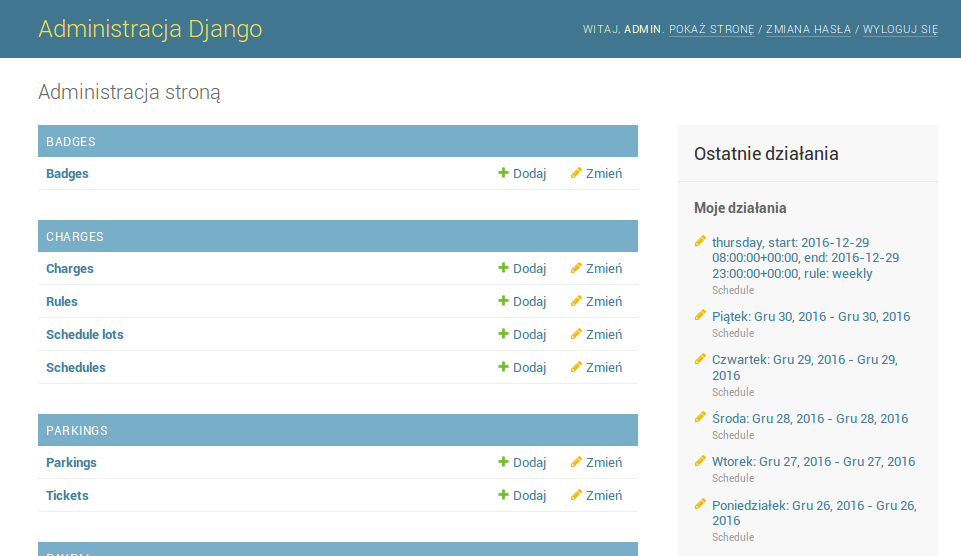
\includegraphics[width=0.9\linewidth]{05/admin_main}
	\end{center}
	\caption{Główny panel administratora}
	\label{serwer_admin}
\end{figure}

\begin{figure}[p]
	\begin{center}
		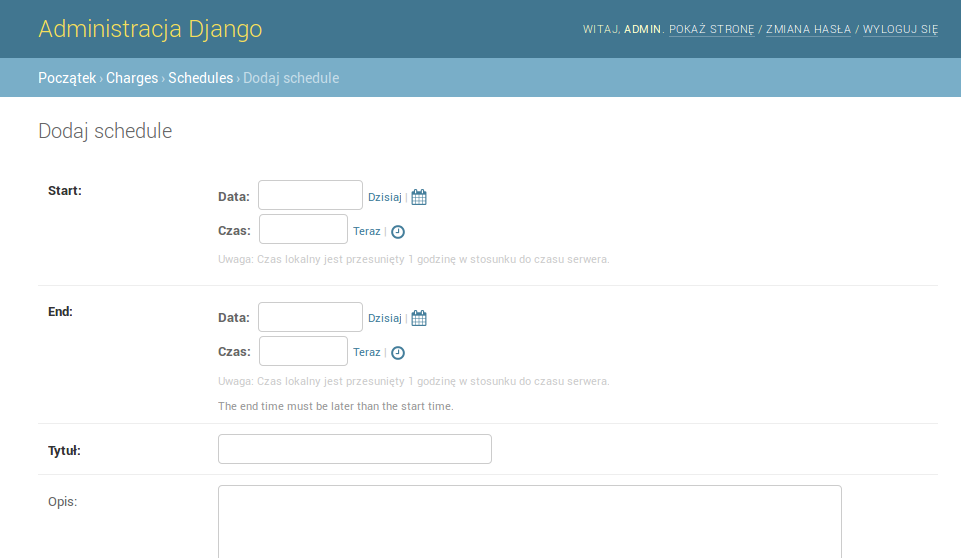
\includegraphics[width=0.9\linewidth]{05/admin_schedule}
	\end{center}
	\caption{Dodawanie nowego grafiku}
	\label{serwer_schedule}
\end{figure}

\clearpage

\subsection{Testy}

Do weryfikowania poprawności tworzonego oprogramowania napisane zostały zestawy testów. Testy jednostkowe sprawdzają odpowiednie funkcjonowanie pojedynczych elementów systemu, takich jak metody klas. Poprawność interakcji zachodzących między modułami sprawdzana jest za pomocą testów integracyjnych. W aplikacji internetowej napisanej w Django, używana do tego celu jest klasa TestCase z pakietu django.test. Każdy z modułów tej aplikacji zawiera plik tests.py, w którym umieszczane są testy. Każdy z nich zawiera przynajmniej jedną asercję, która sprawdza poprawność otrzymanych danych i decyduje o sukcesie lub porażce przeprowadzonego testu. Podobnie sytuacja wygląda w Androidzie, gdzie używana jest biblioteka JUnit. Dodatkowo aplikacja mobilna była testowana zarówno na emulatorze, jak i prawdziwym urządzeniu.
\\
\\
Akceptowanie transakcji przychodzących od klientów systemu wymaga posiadania specjalnego konta sprzedawcy. Dzięki PayPal Sandbox możliwe jest stworzenie środowiska testowego dla aplikacji, w którym mogą być utworzone fikcyjne konta klientów oraz sprzedawców. W ten sposób przeprowadzany jest cały proces płatności, który z perspektywy serwera i aplikacji mobilnej, niczym nie różni się od prawdziwych transakcji. 

\subsection{Środowiska programistyczne i edytory}

Część mobilna systemu została wykonana w Android Studio, będącym dedykowanym środowiskiem programistycznym dla systemu Android. Zostało stworzone przez Google i bazuje na IntelliJ. Jest to rozbudowane IDE, które oprócz tworzenia gotowego szablonu aplikacji, posiada wszystkie funkcje spotykane w nowoczesnych środowiskach, takie jak refaktoryzacja kodu, podpowiedzi, czy poprawianie składni. Razem z nim instalowany jest także emulator, dzięki czemu możliwe jest testowanie aplikacji bez potrzeby posiadania prawdziwego urządzenia z systemem Android.
\\
\\
Do pisania aplikacji serwerowej wykorzystywany był, dostępny z poziomu wiersza poleceń, edytor Vim. Jego standardowa funkcjonalność została rozszerzona o zewnętrzne dodatki, dzięki stworzonemu przez społeczność systemowi zarządzania dodatkami -- Vundle. Dodatek YouCompleteMe wprowadził okna z podpowiedziami i uzupełniania do wpisywanego kodu. Drugi zainstalowanym dodatkiem był NERD Tree, dzięki któremu możliwe stało się wyświetlanie struktury plików katalogu, w którym został uruchomiony edytor.